This sections evaluates the performance of dense Active Appearance Models (dAAMs) built using the proposed methodology in the problem of non-rigid object alignment in-the-wild. Results for four different experiments are reported. Experiments \ref{exp:svs} and \ref{exp:basis} investigate the impact that the Support Vector Shape representation and the subspace constrains for shape flow have, respectively, on the fitting accuracy achieved by dense AAMs build using the proposed pipeline. Experiments \ref{exp:face} and \ref{exp:ear} compare the fitting accuracy of our dense AAMs with respect to that of classic AAMs on the problems of non-rigid face and ear alignment in-the-wild. 
% Finally, experiment \ref{exp:lose} evaluates the effectiveness and performance of the proposed methodology to build dense AAMs of objects that are difficult to annotated with respect to a consistent set of landmarks, such as bottles and human bodies. 
Note that all results reported in this section were obtained by fitting all AAM (dense and classic) using the fast version of the Simultaneous Inverse Compositional algorithm (Fast-SIC) originally proposed by the authors of \cite{Papandreou2008}. For further experimental results and visualizations please refer to our supplementary material. 

%In this section we evaluate the performance of the proposed methodology in a variety of tasks. Results for 4 different experiments are reported. Experiment \ref{exp:1} compares the fitting accuracy of Dense Active Appearance Models (DAAMs) built using our methodology with respect to that of classic AAMs on the problems of non-rigid face and ear alignment in-the-wild. Experiment \ref{exp:2} investigates the impact that the Support Vector Shape representation has on the performance achieved by DAAMs on the the first experiment. Experiment \ref{exp:3} evaluates the effectiveness of the proposed methodology to build DAAMs of objects that are difficult to annotated with respect to a consistent set of landmarks, such as bottles and human bodies. Finally, experiment \ref{exp:4} serves as a qualitative demonstration of how the proposed pipeline can use be effectively used to generate novel modified instances of an object, e.g. caricatures, from simple hand drawn sketches


\subsection{Shape representation}
\label{exp:svs}

This experiment investigates the impact that the SVS representation described in section \ref{sec:svs} has on the final fitting accuracy achieved by dense models built using the propose pipeline. In particular, we compare the SVS representation with a simpler shape representation that consists of directly using binary images obtained from curve line annotations. In order to make the experiment fair we keep all remaining stages of the pipeline intact and simply change between these two shape representations. We use our methodology to build two dense AAMs, one using the SVS representation (SVS-dAAMs) and another using the binary shape representation (Binary-dAAMs). Both models were built using 811 training images of the Labelled Faces Parts in-the-Wild (LFPW) \cite{Belhumeur2011} database and tested on 224 testing images of the same database. We re-annotated all images from this database using the proposed curve line annotation scheme. In order to provide quantitative results, we annotated the reference frame of both dense AAMs (2 images) with the standard 68 point annotation scheme provided by the iBUG group\footnote{\label{ibug_300} \url{http://ibug.doc.ic.ac.uk/resources/300-W/}}. Note that, any set of landmarks annotated on the reference frame can be easily extrapolated to any shape generated by dense shape models.
%; for example, by interpolating its relative position with respect to its immediate reference frame neighbours on the newly generated dense shape instance, \ref{fig:extrapolate_landmarks}. 
Accuracy is reported in terms of the normalized point-to-point error measure described in \cite{Zhu2012}.

The Cumulative Error Distribution (CED) for this experiment is shown in Figure \ref{fig:svs_ced} while fitting statistics are reported in Table \ref{tab:svs_stats}. Looking at the results it can be clearly seen that using SVS results in a constant $\approx$5\% improvement over the simple binary shape representation for almost all CED graph and on the reported fitting statistics.

\begin{figure}[t!]
\centering
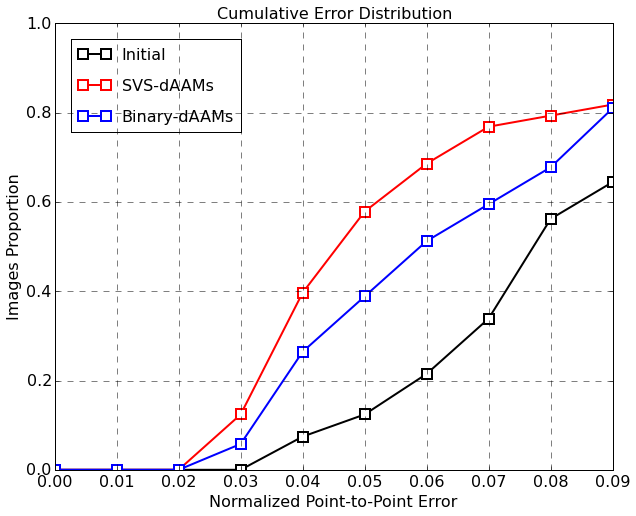
\includegraphics[width=0.42\textwidth]{resources/Fig_SVS/svs_ced}
\caption{CED over 68 landmarks on the LFPW database for experiment \ref{exp:svs}}
\label{fig:svs_ced}
\end{figure}

\begin{table}[t]
\small
\centering
\begin{tabular}{|l|c|c|c|}
\hline
\emph{Method}       & \emph{mean $\pm$ std} & \emph{median} & $\leq 0.05$\\
\hline\hline
Initialization      & 0.0805 $\pm$ 0.0246 & 0.0785 & 12\%\\
SVS                 & 0.0583 $\pm$ 0.0297 & 0.0443 & 57\%\\
Binary              & 0.0640 $\pm$ 0.0300 & 0.0588 & 39\%\\
\hline
\end{tabular}
\caption{Fitting statistics on the LFPW database for experiment \ref{exp:svs}}
\label{tab:svs_stats}
\end{table}

\subsection{Constrained Basis}
\label{exp:basis}

This experiment investigate the impact of introducing subspace constrains for shape flow. The shape representations of training data are independence, thus simply applying flows on shapes breaks the fundamental assumption of motion smoothness. The hypothesis is able to be maintained for shapes as described in section~\ref{sec:trabasis}. To be specific, we take measures of point-to-point error for fitting same data with our pipeline with same configuration, but only alter the low rank basis. 

The experiment results are manifested by constructing two dense AAMs, Basis-dAAMs and no-Basis-dAAMs,among 811 training images from Labelled Faces Parts in-the-Wild (LFPW)\cite{Belhumeur2011} database with 224 testing images using same annotation scheme by iBUG\footnoteref{ibug_300}. 
Cumulative error distributions are shown in Figure~\ref{fig:basis_ced} and corresponding statistics are listed in Table~\ref{tab:basis_stats}. 
It shows shape flow with constrained basis outperforms, constantly, standard flow technique by an unavoidable amount, which significantly supported the necessities of our low rank basis introduced in~\ref{sec:trabasis}.

\begin{figure}[t!]
\centering
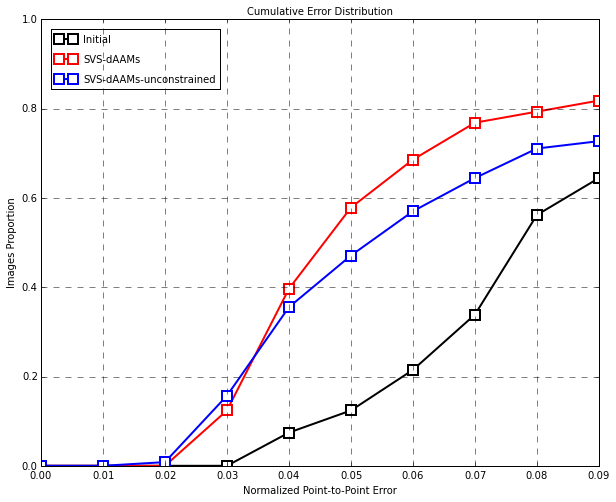
\includegraphics[width=0.42\textwidth]{resources/basis_ced}
\caption{CED over 68 landmarks on the LFPW database for experiment \ref{exp:basis}}
\label{fig:basis_ced}
\end{figure}

\begin{table}[t]
\small
\centering
\begin{tabular}{|l|c|c|c|}
\hline
\emph{Method}       & \emph{mean $\pm$ std} & \emph{median} & $\leq 0.05$\\
\hline\hline
Initialization      & 0.0805 $\pm$ 0.0246 & 0.0785 & 12\%\\
Constrained Flow    & 0.0583 $\pm$ 0.0332 & 0.0443 & 57\%\\
Unconstrained Flow  & 0.0698 $\pm$ 0.0458 & 0.0556 & 46\%\\
\hline
\end{tabular}
\caption{Fitting statistics on the LFPW database for experiment \ref{exp:basis}}
\label{tab:basis_stats}
\end{table}



\subsection{Non-rigid object alignment in-the-wild}
\label{exp:alignment}

In the following set of experiments we use the proposed methodology to build dense AAMs of various object classes (faces, ears, bottles and body pose) and quantitatively asses their respective fitting accuracy when fitted to novel in-the-wild images of the previous objects.

\subsubsection{Face alignment}
\label{exp:face}

This experiment compares the fitting accuracy of our dense AAM versus the one of classic AAM on the problem of non-rigid face alignment in-the-wild. For this experiment, both models were built using the 811 training images of the Labelled Faces Parts in-the-Wild (LFPW) \cite{Belhumeur2011} database. Classic AAM were built from 68 point landmark annotations\footnoteref{ibug_300} using the standard procedure described in \cite{Cootes2001, Matthews2004}; piece-wise affine was used as their motion model. Our dense AAM were built as described in experiment \ref{exp:svs}. Given the evidence obtained from that experiment, we used SVS as the shape representation used throughout our pipeline.

Results for this experiment are reported over the 224 testing images of the LFPW database using again 68 point ground truth landmark annotations\footnoteref{ibug_300}. For this experiment, we report results using two different image representations, \ie pixels intensities (INT) and Histogram of Oriented Gradients (HOG) \cite{Dalal2005} for both models. The two techniques were initialized using our own version of the face detector described in \cite{Zhu2012}.

Cumulative Error Distributions (CED) for this experiment are shown in Figure \ref{fig:face_ced} while fitting statistics are reported in Table \ref{tab:face_stats}. Results show that, for this experiment, the fitting accuracy achieved by our dense AAM is comparable to the one achieved by classic AAMs using both image representations. In particular, our method seems to perform marginally better when pixel intensities are used as the image representation, while classic AAMs slightly outperform our technique for HOG. Overall, both methods achieve similar performance for errors below 5\%. We believe this results are remarkable, provided that our model was learned from curve annotations ($\approx$ 30 seconds/image) instead of expensive point landmark annotations ($\approx$ 4 minutes/image).

\begin{figure}[t!]
\centering
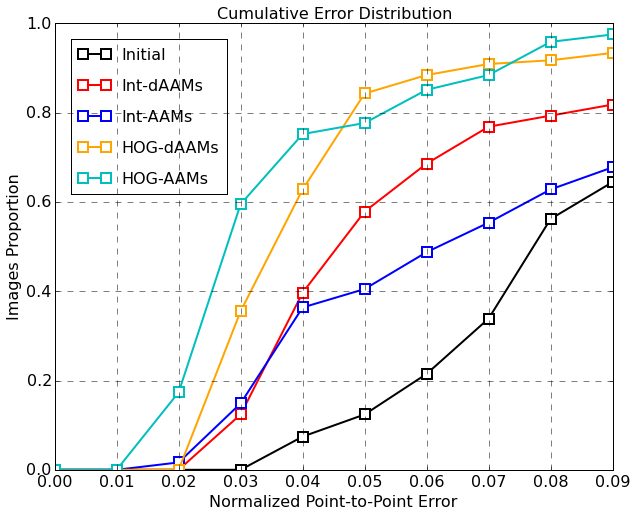
\includegraphics[width=0.42\textwidth]{resources/Fig_Alignment/face_ced}
\caption{CED over 68 landmarks on the LFPW database for experiment \ref{exp:face}}
\label{fig:face_ced}
\end{figure}

\begin{table}[t]
\small
\centering
\begin{tabular}{|l|c|c|c|}
\hline
\emph{Method}   & \emph{mean $\pm$ std} & \emph{median} & $\leq 0.05$\\
\hline\hline
Initialization  & 0.0805 $\pm$ 0.0246 & 0.0785 & 12\%\\
INT - dAAM      & 0.0583 $\pm$ 0.0332 & 0.0443 & 57\%\\
INT - AAM       & 0.0876 $\pm$ 0.0608 & 0.0797 & 40\%\\
HOG - dAAM      & 0.0413 $\pm$ 0.0212 & 0.0340 & 85\%\\
HOG - AAM       & 0.0354 $\pm$ 0.0210 & 0.0266 & 77\%\\
\hline
\end{tabular}
\caption{Fitting statistics on the LFPW database for experiment \ref{exp:face}}
\label{tab:face_stats}
\end{table}

\subsubsection{Ear alignment}
\label{exp:ear}

In this experiment, we studied the feasibility of building and fitting statistical deformable models that capture the variability of the human ear. To this end, we collected 605 high resolution images of ears in unconstrained scenarios and annotated them using both a newly defined 55 point annotation scheme for ears and the curve annotations proposed in this paper. Examples of these two type of ear annotations are shown in Figure \ref{fig:intro}. We randomly split the previous database into two disjoint sets of training (500) and testing (105) images. We compare the fitting accuracy obtained by our dense AAM model versus the one of classic AAM on these data. Both models were built using the 500 images on the previous training set and their fitting accuracy evaluated on the 105 images of the testing set. Note here that we used the same procedures used in experiment \ref{exp:svs} to build the models and evaluate the results (piece-wise affine motion model for classic AAM and SVS, constrained flow and landmark interpolation for dense AAM).

Results for this experiments are shown in Figure \ref{fig:ear_ced} and Table \ref{tab:ear_stats}. In this case, we can readily observe that the accuracy achieved by ear models, in terms of the previous normalized point-to-point error measure, is lower than the one achieved by face models. This result is expected due to the more complex structure of the ear shape. Through visual inspection we determined that fitting errors below $0.1$ for ears typically look plausible under the previous error measure \ref{fig:ear_error}. Results for this experiment show that our approach performs significantly better than the classic AAM when pixels intensities are used as image representation. In fact, classic AAM fail to improve the accuracy of the original initialization on $\approx45\%$ of the test images while for our the case of our dense model this number goes up to $\approx70\%$. On the other hand, the accuracy of both models dramatically improves using HOG. In this case, classic AAM outperform our dense AAM for small errors up to $0.1$ while both models obtain similar results for errors around $0.1$. Again, the fact that the propose pipeline is capable of dealing with the complex structure of the ear shape and learn dense AAM from simple curve line annotations that can compete and even surpass (in the case of a simple pixel intensity image representation) classic AAM, build from carefully annotated point landmarks, is quite remarkable. 

\begin{figure}[t!]
\centering
    \begin{subfigure}[b]{0.115\textwidth}
            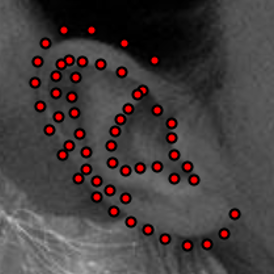
\includegraphics[height=1\textwidth]{resources/Fig_Alignment/ear_06_55}
    \caption{$0.06$}
    \end{subfigure}
    \begin{subfigure}[b]{0.115\textwidth}
            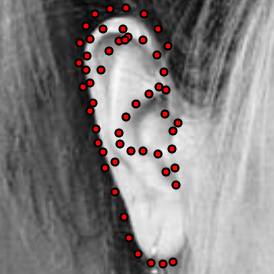
\includegraphics[height=1\textwidth]{resources/Fig_Alignment/ear_1_55}
    \caption{$0.1$}
    \end{subfigure}
    \begin{subfigure}[b]{0.115\textwidth}
            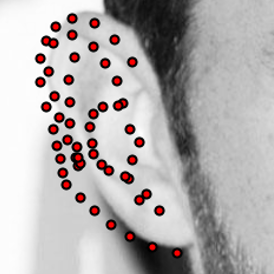
\includegraphics[height=1\textwidth]{resources/Fig_Alignment/ear_14_55}
    \caption{$0.14$}
    \end{subfigure}
    \begin{subfigure}[b]{0.115\textwidth}
            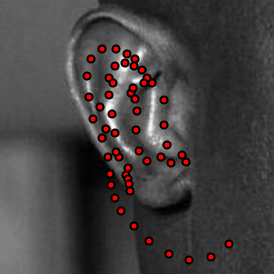
\includegraphics[height=1\textwidth]{resources/Fig_Alignment/ear_23_55}
    \caption{$0.23$}
    \end{subfigure}
\caption{Qualitative examples showing different values of normalize point-to-point error measure for ears.}
\label{fig:ear_error}
\end{figure}

\begin{figure}[t!]
\centering
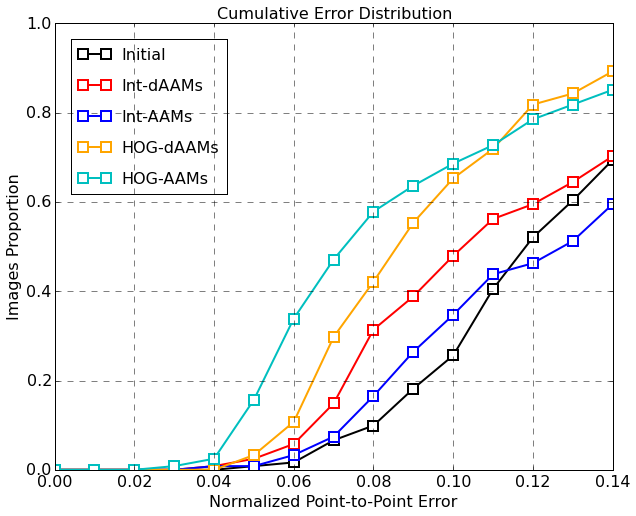
\includegraphics[width=0.42\textwidth]{resources/Fig_Alignment/ear_ced}
\caption{CED over 55 landmarks on the collected ear database for experiment \ref{exp:ear}}
\label{fig:ear_ced}
\end{figure}

\begin{table}[t]
\small
\centering
\begin{tabular}{|l|c|c|c|}
\hline
\emph{Method}   & \emph{mean $\pm$ std} & \emph{median} & $\leq 0.1$\\
\hline\hline
Initialization  & 0.1246 $\pm$ 0.0394 & 0.1186 & 32\%\\
INT - dAAM      & 0.1180 $\pm$ 0.0533 & 0.1030 & 47\%\\
INT - AAM       & 0.1332 $\pm$ 0.0547 & 0.1261 & 35\%\\
HOG - dAAM      & 0.0967 $\pm$ 0.0436 & 0.0856 & 66\%\\
HOG - AAM       & 0.0908 $\pm$ 0.0522 & 0.0729 & 69\%\\
\hline
\end{tabular}
\caption{Fitting statistics on the collected ear database for experiment \ref{exp:ear}}
\label{tab:ear_stats}
\end{table}


% \subsubsection{Object alignment with loosely defined landmarks}
% \label{exp:lose}

% In this section, we experimenting on utilising our dense AAM for objects segmentation. Two subjects, bottles and human, are involved. As for human segmentation, we gather ground true images from Space-Time Actions\footnote{\label{sta} \url{http://www.wisdom.weizmann.ac.il/~vision/SpaceTimeActions.html}}\cite{ActionsAsSpaceTimeShapes_iccv05]}, where several human action sequences are provided with segmentation. There are 10 categories actions where each category contains 10 subjects each are recorded with more than 120 frames. For bottles, 500 high resolution images of bottles are collected and annotated using not only a newly defined 50 point annotation scheme for bottles, but also the curve annotations proposed in this paper. Figure \ref{fig:intro} demonstrated different annotations of both bottles and human actions. We randomly split the previous database into two disjoint sets of training (500) and testing (105) images. We compare the fitting accuracy obtained by our dense AAM model versus the one of classic AAM on these data. Both models were built using the 500 images on the previous training set and their fitting accuracy evaluated on the 105 images of the testing set. Note here that we used the same procedures used in experiment \ref{exp:1} to build the models and evaluate the results (piece-wise affine motion model for classic AAM and SVS, constrained flow and landmark interpolation for dense AAM).


%\subsection{DAAMs without consistent annotations}
%\label{exp:3}

%\subsection{Object generation from sketches}
%\label{exp:4}

%\begin{figure}[h!]
%    \centering
%    \includegraphics[width=0.45\textwidth]{resources/Fig_Draw/draw}
%    \caption{Figure}
%    \label{fig:draw}
%\end{figure}

% \clearpage

%\begin{figure}[h!]
%    \centering
%    \begin{subfigure}[b]{0.45\textwidth}
%        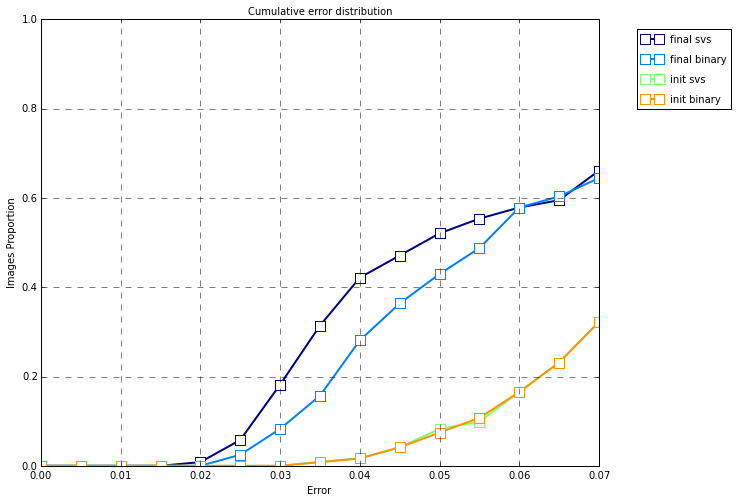
\includegraphics[width=\textwidth]{resources/Fig_SVS/faces_svs_binary_gaussian}
%        \caption{AAM Principle Components Contribution}
%    \end{subfigure}
%    \hfill
%    \begin{subfigure}[b]{0.2\textwidth}
%            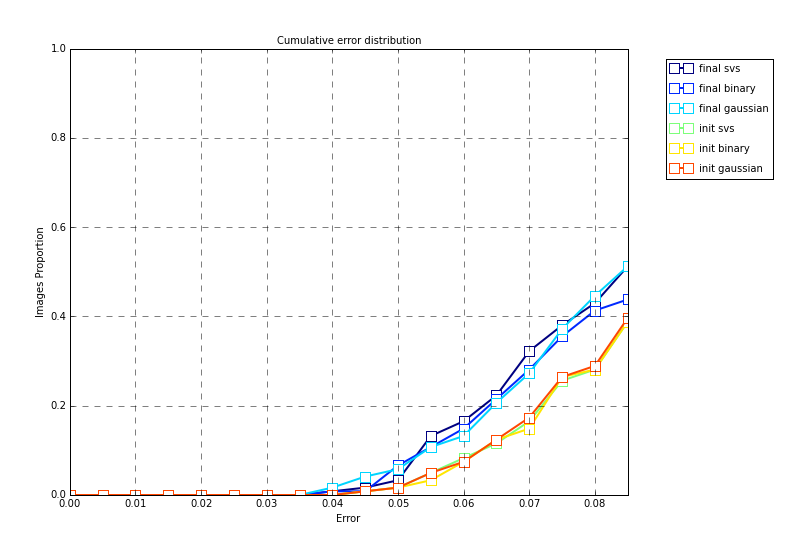
\includegraphics[width=\textwidth]{resources/Fig_SVS/ears_svs_binary_gaussian}
%        % \caption{Shape Flow Principle Components Contribution}
%    \end{subfigure}
%    \\
%    \begin{subfigure}[b]{0.2\textwidth}
%            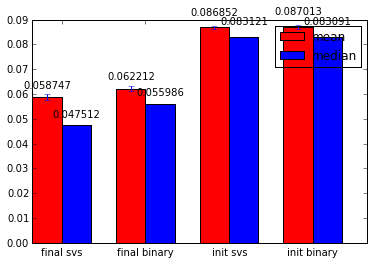
\includegraphics[width=\textwidth]{resources/Fig_SVS/faces_svs_binary_gaussian_statistics}
%        % \caption{AAM Principle Components Contribution}
%    \end{subfigure}
%    \hfill
%    \begin{subfigure}[b]{0.2\textwidth}
%            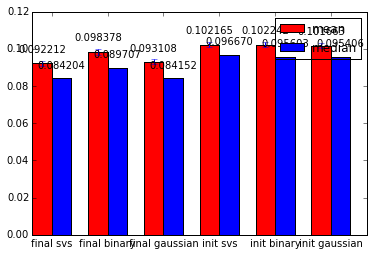
\includegraphics[width=\textwidth]{resources/Fig_SVS/ears_svs_binary_gaussian_statistics}
%        % \caption{Shape Flow Principle Components Contribution}
%    \end{subfigure}
%    \caption{Principle Components Contribution}
%\end{figure}


%\begin{figure}[h!]
%    \centering
%    \begin{subfigure}[b]{0.2\textwidth}
%            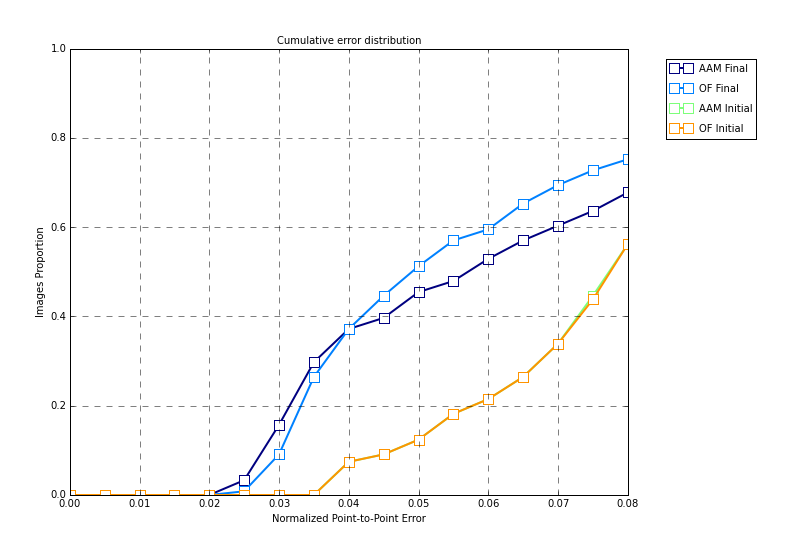
\includegraphics[width=\textwidth]{resources/Fig_Alignment/face_intensity}
%        % \caption{AAM Principle Components Contribution}
%    \end{subfigure}
%    \hfill
%    \begin{subfigure}[b]{0.2\textwidth}
%            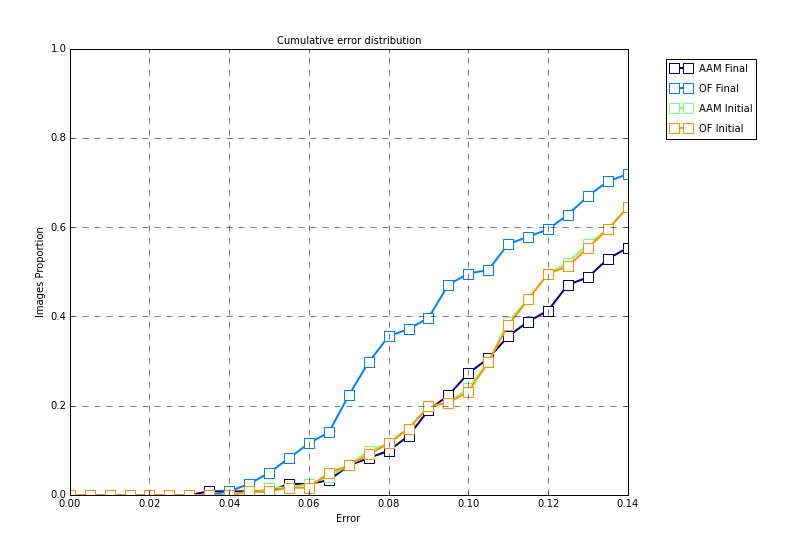
\includegraphics[width=\textwidth]{resources/Fig_Alignment/ear_intensity}
%        % \caption{Shape Flow Principle Components Contribution}
%    \end{subfigure}
%    \\
%    \begin{subfigure}[b]{0.2\textwidth}
%            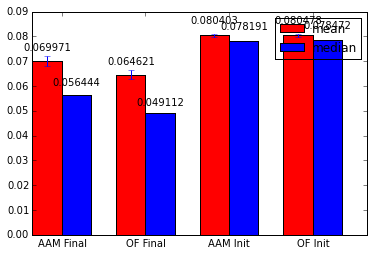
\includegraphics[width=\textwidth]{resources/Fig_Alignment/face_intensity_statistics}
%        % \caption{AAM Principle Components Contribution}
%    \end{subfigure}
%    \hfill
%    \begin{subfigure}[b]{0.2\textwidth}
%            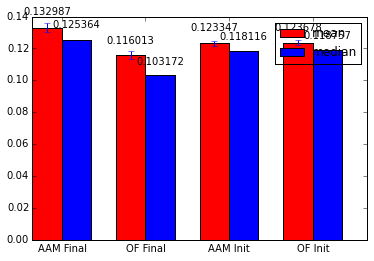
\includegraphics[width=\textwidth]{resources/Fig_Alignment/ear_intensity_statistics}
%        % \caption{Shape Flow Principle Components Contribution}
%    \end{subfigure}
%    \caption{CED Plot and Statistics of Comparison with Classic AAM}
%\end{figure}